\documentclass[11pt,a4paper]{article}

\usepackage[T1]{fontenc}
\usepackage[utf8]{inputenc}
\usepackage{lmodern}
\usepackage[margin=2.5cm]{geometry}
\usepackage{microtype}
\usepackage{amsmath,amssymb}
\usepackage{booktabs}
\usepackage{array}
\usepackage{enumitem}
\usepackage{tikz}
\usetikzlibrary{decorations.pathreplacing}
\usepackage{xcolor}
\usepackage[hidelinks]{hyperref}

\setlist[itemize]{topsep=0.35em,itemsep=0.2em}
\setlist[enumerate]{topsep=0.35em,itemsep=0.25em}

\hypersetup{
  pdftitle={Truncated SHA-2: Collision Resistance and Digital Signatures},
  pdfauthor={Data Security}
}

\newcommand{\Hn}{H_{n}}
\newcommand{\prefix}{\operatorname{prefix}}

\title{%
  Truncated SHA-2\\[0.35em]
  \large Collision Resistance of Prefixes and Digital Signatures%
}
\author{Data Security}
\date{\today}

\begin{document}
\maketitle
\thispagestyle{empty}

\begin{abstract}
\noindent
A system that accepts a SHA-256 digest after keeping only its most significant
\(n\) bits has a much smaller collision bound than the full hash.
This note states the assignment: measure that loss, and judge what it means
for a digital signature computed on the truncated digest.
The concrete setting is the poisoned-message story of Alice and her employer,
replayed for \(\Hn\) instead of MD5.
\end{abstract}

\section{Your mission}

\begin{enumerate}
  \item Replay Alice's investigation and determine how secure the truncated
        hash function, and the digital signature on top of it, really are.
  \item Find a realistic attack against meaningful messages.
        The construction itself will be covered in a later lecture.
\end{enumerate}

The reference story is Daum and Lucks,
\textit{Hash Collisions (The Poisoned Message Attack)}:
\begin{center}
\url{https://www.sos.cs.ru.nl/applications/courses/security2015/md5collisions/index.html}
\end{center}

In that story Alice prepares two PostScript documents that display different
text (a letter of recommendation, and an order granting her access) but share
one MD5 digest:
\begin{center}
\texttt{a25f7f0b29ee0b3968c860738533a4b9}
\end{center}
A signature on the letter is therefore a valid signature on the order.
The question here is the same one, asked of a prefix of SHA-256:
once only \(n\) bits are checked, which pairs of messages become practical to
find, and when does a signature on \(\Hn(x)\) stop distinguishing them?

\section{What is SHA-2?}

SHA-2 is a family of cryptographic hash functions standardized by NIST:
SHA-224, SHA-256, SHA-384, and SHA-512.
The functions are designed to be collision-resistant and preimage-resistant.
They are widely used in digital signatures, TLS, and blockchain systems.

This assignment truncates SHA-256.
Write \(H(x)\) for the full 256-bit digest of a message \(x\).
A truncated check keeps the most significant \(n\) bits and discards the rest:
\begin{equation}
  \Hn(x) = \prefix_{n}\bigl(H(x)\bigr).
  \label{eq:trunc}
\end{equation}
The prefix is shorter than \(H(x)\), so distinct messages collide under
\(\Hn\) more easily than under \(H\).
Truncation reduces collision resistance.

When a digest is written in hexadecimal, the leading digits are the most
significant bits.
For \(n\) a multiple of \(4\), \(\Hn(x)\) is the first \(n/4\) hex digits of
\(H(x)\).

\section{Most and least significant bits}
\label{sec:msb}

Bits of a byte are written left to right, from the most significant bit
(MSB) to the least significant bit (LSB).
Figure~\ref{fig:msb} uses the same example as the lecture,
the byte \texttt{01100100}.

\begin{figure}[ht]
  \centering
  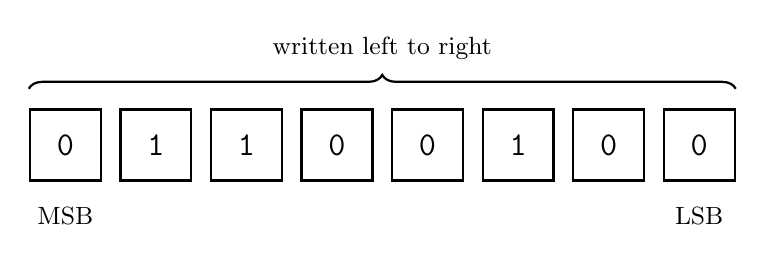
\begin{tikzpicture}[
      bit/.style={draw, thick, minimum size=9mm, inner sep=0pt,
                  font=\ttfamily\large},
      bitlabel/.style={font=\small}
    ]
    \foreach \bit [count=\i from 0] in {0,1,1,0,0,1,0,0}{
      \node[bit] (b\i) at (1.15*\i,0) {\bit};
    }
    \node[bitlabel, anchor=north] at ([yshift=-2mm]b0.south) {MSB};
    \node[bitlabel, anchor=north] at ([yshift=-2mm]b7.south) {LSB};
    \draw[decorate, decoration={brace, amplitude=5pt}, thick]
      ([yshift=2.5mm]b0.north west) -- ([yshift=2.5mm]b7.north east)
      node[midway, above=7pt, font=\small] {written left to right};
  \end{tikzpicture}
  \caption{One byte, most significant bit on the left.
           \(\prefix_{n}\) keeps the leftmost \(n\) bits of this ordering,
           scaled up to the 256-bit SHA-256 digest.}
  \label{fig:msb}
\end{figure}

\begin{table}[ht]
  \centering
  \caption{Names of the bits in \texttt{01100100}.
           Place values show why the left-hand bits dominate the integer
           value of the byte (\(64 + 32 + 4 = 100\)).}
  \label{tab:bits}
  \begin{tabular}{@{}cccc@{}}
    \toprule
    From the left & Bit & Place value & Name \\
    \midrule
    1 & 0 & \(2^{7}\) & Most significant bit \\
    2 & 1 & \(2^{6}\) & 2nd most significant bit \\
    3 & 1 & \(2^{5}\) & 3rd most significant bit \\
    4 & 0 & \(2^{4}\) & 4th most significant bit \\
    5 & 0 & \(2^{3}\) & 5th most significant bit \\
    6 & 1 & \(2^{2}\) & 6th most significant bit \\
    7 & 0 & \(2^{1}\) & 7th most significant bit \\
    8 & 0 & \(2^{0}\) & Least significant bit \\
    \bottomrule
  \end{tabular}
\end{table}

The same left-to-right convention applies to a SHA-256 digest.
\(\Hn(x)\) in \eqref{eq:trunc} is the block of \(n\) bits that starts at the
MSB and runs toward the LSB.
The discarded bits are the less significant tail.

\section{Collision-attack complexity}

A collision is a pair of distinct inputs with the same truncated digest:
\[
  x \neq x' \quad\text{and}\quad \Hn(x) = \Hn(x').
\]
The best known generic attack is still the birthday attack.
Its cost is
\begin{equation}
  \boxed{\,O\bigl(2^{n/2}\bigr)\,}
  \label{eq:birthday}
\end{equation}
Truncation therefore gives at most \(n/2\) bits of collision security.
A full SHA-256 digest has \(n = 256\), and the same bound is \(2^{128}\).
Every bit dropped from the prefix cuts the birthday cost in half.

\section{Security implications}

\begin{itemize}
  \item Short prefixes allow practical collisions.
        The lecture's examples are \(n = 32\) and \(n = 64\),
        with birthday costs \(2^{16}\) and \(2^{32}\).
  \item The truncated check is safe only when \(n\) is sufficiently large.
        The lecture's example threshold is \(n \ge 128\),
        which leaves a birthday cost of at least \(2^{64}\).
\end{itemize}

A signature that covers \(\Hn(x)\) and ignores the remaining
\(256 - n\) bits accepts every message that lands in the same prefix.
The signature is only as collision-resistant as \(\Hn\).

\section{Required work}

The experimental part of the assignment is a collision search on
\(\Hn\). Include all of the following.

\begin{enumerate}
  \item Find the largest \(n\) you can reach.
        Begin at \(n = 32\) and move upward.
  \item Find as many approaches as you can.
        The hinted starting points are a hash table and Floyd's
        cycle-finding algorithm.
  \item Trade computation against memory, and parallelize the search.
        Report what each approach stores, how much work it does, and
        where the machine actually runs out of time or memory.
\end{enumerate}

For each \(n\) you reach, record a concrete colliding pair and the shared
prefix, together with the time and memory of the run.
The interesting comparison is across methods at the same \(n\):
a hash table spends memory to detect a repeated prefix quickly,
while a cycle-finding search stores a constant amount of state and
pays for that with more hashing.

\section{Goal of this topic}

Understand how truncating SHA-2 outputs affects collision resistance,
and why birthday-bound attacks dominate the analysis.
The generic cost \eqref{eq:birthday} is the yardstick:
an attack that beats it on \(\Hn\) would be a cryptanalytic result about
SHA-256 itself, and a search that only matches it is still enough to show
that a short prefix, and any signature reduced to that prefix, is weak.

The later lecture on meaningful messages asks for a collision the way Alice's
is a collision: two inputs a person would accept as different documents,
sharing \(\Hn\), so that one signature verifies on both.
Until that construction is given, the measurement above is the evidence
for the security conclusion.

\begin{thebibliography}{9}
\bibitem{daum-lucks}
Magnus Daum and Stefan Lucks.
\newblock Hash Collisions (The Poisoned Message Attack).
\newblock Mirror used in the Security course at Radboud University,
\newblock \url{https://www.sos.cs.ru.nl/applications/courses/security2015/md5collisions/index.html}.

\bibitem{fips180-4}
National Institute of Standards and Technology.
\newblock \emph{Secure Hash Standard (SHS)}, FIPS PUB 180-4, 2015.
\end{thebibliography}

\end{document}
